% !Mode:: "TeX:UTF-8"

\documentclass[12pt,openany,oneside]{book}

\input{setup/package} % 定义所需宏包

\begin{document}
% !Mode:: "TeX:UTF-8"
% Author: Unlucky
% Blog: http://unlucky.orgfree.com/blog

%%%%%%%%%% Fonts Definition and Basics %%%%%%%%%%%%%%%%%
\XeTeXlinebreaklocale "zh"
\XeTeXlinebreakskip = 0pt plus 1pt minus 0.1pt
\setCJKfamilyfont{song}{SimSun}             % 宋体
\newcommand{\song}{\CJKfamily{song}}
\setCJKfamilyfont{fs}{FangSong}             % 仿宋体
\newcommand{\fs}{\CJKfamily{fs}}
\setCJKfamilyfont{kai}{KaiTi}               % 楷体
\newcommand{\kai}{\CJKfamily{kai}}
\setCJKfamilyfont{hei}{SimHei}              % 黑体
\newcommand{\hei}{\CJKfamily{hei}}
\setCJKfamilyfont{li}{LiSu}                 % 隶书
\newcommand{\li}{\CJKfamily{li}}
\setCJKfamilyfont{tnroman}{Times New Roman} % Times New Roman
\newcommand{\tnroman}{\CJKfamily{tnroman}}

\newcommand{\yihao}{\fontsize{26pt}{26pt}\selectfont}       % 一号, 单倍行距
\newcommand{\xiaoyi}{\fontsize{24pt}{24pt}\selectfont}      % 小一, 单倍行距
\newcommand{\erhao}{\fontsize{22pt}{27.5pt}\selectfont}       % 二号, 1.25倍行距
\newcommand{\xiaoer}{\fontsize{18pt}{18pt}\selectfont}      % 小二, 单倍行距
\newcommand{\sanhao}{\fontsize{16pt}{16pt}\selectfont}      % 三号, 单倍行距
\newcommand{\xiaosan}{\fontsize{15pt}{22.5pt}\selectfont}     % 小三, 单倍行距
\newcommand{\sihao}{\fontsize{14pt}{14pt}\selectfont}       % 四号, 单倍行距
\newcommand{\xiaosi}{\fontsize{12pt}{18pt}\selectfont}      % 小四, 单倍行距
\newcommand{\wuhao}{\fontsize{10.5pt}{10.5pt}\selectfont}   % 五号, 单倍行距
\newcommand{\xiaowu}{\fontsize{9pt}{9pt}\selectfont}        % 小五, 单倍行距

\setCJKmainfont{SimSun}
\setCJKmonofont{SimSun}
\setmainfont{Times New Roman}

% \CJKcaption{gb_452}
% \CJKtilde  % 重新定义了波浪符~的意义
\newcommand\prechaptername{第}
\newcommand\postchaptername{章}

% \punctstyle{plain}
% 调整罗列环境的布局
\setitemize{leftmargin=3em,itemsep=0em,partopsep=0em,parsep=0em,topsep=-0em}
\setenumerate{leftmargin=3em,itemsep=0em,partopsep=0em,parsep=0em,topsep=0em}
% \setlength{\baselineskip}{20pt}
% \renewcommand{\baselinestretch}{1.38} % 设置行距

% 避免宏包 hyperref 和 arydshln 不兼容带来的目录链接失效的问题。
\def\temp{\relax}
\let\temp\addcontentsline
\gdef\addcontentsline{\phantomsection\temp}

% 自定义项目列表标签及格式 \begin{publist} 列表项 \end{publist}
\newcounter{pubctr} %自定义新计数器
\newenvironment{publist}{%%%%%定义新环境
  \begin{list}{[\arabic{pubctr}]} %%标签格式
    {
      \usecounter{pubctr}
      \setlength{\leftmargin}{2.5em}   % 左边界 \leftmargin =\itemindent + \labelwidth + \labelsep
      \setlength{\itemindent}{0em}     % 标号缩进量
      \setlength{\labelsep}{1em}       % 标号和列表项之间的距离,默认0.5em
      \setlength{\rightmargin}{0em}    % 右边界
      \setlength{\topsep}{0ex}         % 列表到上下文的垂直距离
      \setlength{\parsep}{0ex}         % 段落间距
      \setlength{\itemsep}{0ex}        % 标签间距
      \setlength{\listparindent}{0pt} % 段落缩进量
    }}
  {\end{list}}%%%%%

\makeatletter
\renewcommand\normalsize{
  \@setfontsize\normalsize{12pt}{12pt} % 小四对应12pt
  \setlength\abovedisplayskip{4pt}
  \setlength\abovedisplayshortskip{4pt}
  \setlength\belowdisplayskip{\abovedisplayskip}
  \setlength\belowdisplayshortskip{\abovedisplayshortskip}
  \let\@listi\@listI}
\def\defaultfont{\renewcommand{\baselinestretch}{1.38}\normalsize\selectfont}
% 设置行距和段落间垂直距离
\renewcommand{\CJKglue}{\hskip 0.96pt plus 0.08\baselineskip} %加大字间距,使每行33个字

\makeatother
%%%%%%%%%%%%% Contents %%%%%%%%%%%%%%%%%
% 主目录设置
\renewcommand{\contentsname}{目\qquad 录}
\setcounter{tocdepth}{1}
\titlecontents{chapter}[2em]{\vspace{.5\baselineskip}\xiaosan\song}%
{\prechaptername\CJKnumber{\thecontentslabel}\postchaptername\qquad}{} %
{\hspace{.5em}\titlerule*[10pt]{$\cdot$}\sihao\contentspage}
\titlecontents{section}[3em]{\vspace{.25\baselineskip}\sihao\song} %
{\thecontentslabel\quad}{} %
{\hspace{.5em}\titlerule*[10pt]{$\cdot$}\sihao\contentspage}
\titlecontents{subsection}[4em]{\vspace{.25\baselineskip}\xiaosi\song} %
{\thecontentslabel\quad}{} %
{\hspace{.5em}\titlerule*[10pt]{$\cdot$}\sihao\contentspage}

% 图目录设置
\renewcommand{\listfigurename}{图目录}
\newcommand{\loflabel}{图}
\renewcommand{\numberline}[1]{\loflabel~#1\hspace*{1em}}

% 表目录设置
\renewcommand{\listtablename}{表目录}
\newcommand{\lotlabel}{表}
\renewcommand{\numberline}[1]{\lotlabel~#1\hspace*{1em}}


%%%%%%%%%% Chapter and Section %%%%%%%%%%%%%%%%%
\setcounter{secnumdepth}{4}
\setlength{\parindent}{2em}
\renewcommand{\chaptername}{\prechaptername\CJKnumber{\thechapter}\postchaptername}
\titleformat{\chapter}{\centering\xiaosan\bfseries}{\chaptername}{2em}{}
\titlespacing{\chapter}{0pt}{0.3\baselineskip}{1\baselineskip}
\titleformat{\section}{\sihao\bfseries}{\thesection}{1em}{}
\titlespacing{\section}{0pt}{0.2\baselineskip}{0.5\baselineskip}
\titleformat{\subsection}{\sihao\bfseries}{\thesubsection}{1em}{}
\titlespacing{\subsection}{0pt}{0.1\baselineskip}{0.3\baselineskip}
\titleformat{\subsubsection}{\sihao\bfseries}{\thesubsubsection}{1em}{}
\titlespacing{\subsubsection}{0pt}{0}{0}

%%%%%%%%%% Table, Figure and Equation %%%%%%%%%%%%%%%%%
\renewcommand{\tablename}{表} % 插表题头
\renewcommand{\figurename}{图} % 插图题头
\renewcommand{\thefigure}{\arabic{chapter}-\arabic{figure}} % 使图编号为 7-1 的格式 %\protect{~}
\renewcommand{\thesubfigure}{\alph{subfigure})}%使子图编号为 a)的格式
\renewcommand{\thesubtable}{(\alph{subtable})} %使子表编号为 a)的格式
\renewcommand{\thetable}{\arabic{chapter}-\arabic{table}}%使表编号为 7-1 的格式
\renewcommand{\theequation}{\arabic{chapter}-\arabic{equation}}%使公式编号为 7-1 的格式

%% 定制浮动图形和表格标题样式
\makeatletter
\long\def\@makecaption#1#2{%
  \vskip\abovecaptionskip
  \sbox\@tempboxa{\centering\wuhao\song{#1\qquad #2} }%
  \ifdim \wd\@tempboxa >\hsize
  \centering\wuhao\song{#1\qquad #2} \par
  \else
  \global \@minipagefalse
  \hb@xt@\hsize{\hfil\box\@tempboxa\hfil}%
  \fi
  \vskip\belowcaptionskip}
\makeatother
\captiondelim{~~~~} %用来控制longtable表头分隔符

%%%%%%%%%% Theorem Environment %%%%%%%%%%%%%%%%%
\theoremstyle{plain}
\theorembodyfont{\song\rmfamily}
\theoremheaderfont{\hei\rmfamily}
\newtheorem{theorem}{定理~}[chapter]
\newtheorem{lemma}{引理~}[chapter]
\newtheorem{axiom}{公理~}[chapter]
\newtheorem{proposition}{命题~}[chapter]
\newtheorem{corollary}{推论~}[chapter]
\newtheorem{definition}{定义~}[chapter]
\newtheorem{conjecture}{猜想~}[chapter]
\newtheorem{example}{例~}[chapter]
\newtheorem{remark}{注~}[chapter]
\newtheorem{algorithm}{算法~}[chapter]
\newenvironment{proof}{\noindent{\hei 证明:}}{\hfill $ \square $ \vskip 4mm}
\theoremsymbol{$\square$}

%%%%%%%%%% Page: number, header and footer  %%%%%%%%%%%%%%%%%

% \frontmatter 或 \pagenumbering{roman}
% \mainmatter 或 \pagenumbering{arabic}
\makeatletter
\renewcommand\frontmatter{\clearpage
  \@mainmatterfalse
  \pagenumbering{Roman}} % 正文前罗马字体编号
\makeatother


%%%%%%%%%% References %%%%%%%%%%%%%%%%%
\renewcommand{\bibname}{参考文献}
% 重定义参考文献样式,来自thu
\makeatletter
\renewenvironment{thebibliography}[1]{%
  \titleformat{\chapter}{\raggedright\sihao\hei}{\chaptername}{2em}{}
  \chapter*{\bibname}%
  \wuhao
  \list{\@biblabel{\@arabic\c@enumiv}}%
  {\renewcommand{\makelabel}[1]{##1\hfill}
    \settowidth\labelwidth{0.5cm}
    \setlength{\labelsep}{0pt}
    \setlength{\itemindent}{0pt}
    \setlength{\leftmargin}{\labelwidth+\labelsep}
    \addtolength{\itemsep}{-0.7em}
    \usecounter{enumiv}%
    \let\p@enumiv\@empty
    \renewcommand\theenumiv{\@arabic\c@enumiv}}%
  \sloppy\frenchspacing
  \clubpenalty4000%
  \@clubpenalty \clubpenalty
  \widowpenalty4000%
  \interlinepenalty4000%
  \sfcode`\.\@m}
{\def\@noitemerr
  {\@latex@warning{Empty `thebibliography' environment}}%
  \endlist\frenchspacing}
\makeatother

\addtolength{\bibsep}{-0.5em} % 缩小参考文献间的垂直间距
\setlength{\bibhang}{2em} %每个条目自第二行起缩进的距离

% 参考文献引用作为上标出现
% \newcommand{\citeup}[1]{\textsuperscript{\cite{#1}}}
\makeatletter
\def\@cite#1#2{\textsuperscript{[{#1\if@tempswa , #2\fi}]}}
\makeatother
%% 引用格式
\bibpunct{[}{]}{,}{s}{}{,}

%%%%%%%%%% Cover %%%%%%%%%%%%%%%%%
% 封面、摘要、版权、致谢格式定义
\makeatletter
\def\ctitle#1{\def\@ctitle{#1}}\def\@ctitle{}
\def\caffil#1{\def\@caffil{#1}}\def\@caffil{}
\def\csubject#1{\def\@csubject{#1}}\def\@csubject{}
\def\cauthor#1{\def\@cauthor{#1}}\def\@cauthor{}
\def\csupervisor#1{\def\@csupervisor{#1}}\def\@csupervisor{}
\def\cdate#1{\def\@cdate{#1}}\def\@cdate{}
\long\def\cabstract#1{\long\def\@cabstract{#1}}\long\def\@cabstract{}
\long\def\eabstract#1{\long\def\@eabstract{#1}}\long\def\@eabstract{}
\def\ckeywords#1{\def\@ckeywords{#1}}\def\@ckeywords{}
\def\ekeywords#1{\def\@ekeywords{#1}}\def\@ekeywords{}
\def\cheading#1{\def\@cheading{#1}}\def\@cheading{}

% 在book文件类别下,\leftmark自动存录各章之章名,\rightmark记录节标题
\pagestyle{fancy}
% 去掉章节标题中的数字 务必放到\pagestyle{fancy}之后才会起作用
%% 不要注销这一行,否则页眉会变成:“第1章1  绪论”样式
\renewcommand{\chaptermark}[1]{\markboth{\chaptername~\ #1}{}}
\fancyhf{}
% \fancyhead[C]{\song\wuhao \leftmark} % 页眉显示章节名称
\fancyhead[C]{\song\xiaowu \@cheading}
% \fancyhead[CO]{\song\wuhao \@cheading}
% \fancyhead[CE]{\song\wuhao \@cheading}
\fancyfoot[C]{\song\xiaowu ~\thepage~}

\fancypagestyle{plain}{% 设置开章页页眉页脚风格
  \fancyhf{}%
  % \fancyhead[C]{\song\wuhao \leftmark}
  \fancyhead[C]{\song\xiaowu \@cheading}
  \fancyfoot[C]{\song\xiaowu ~\thepage~ } %%首页页脚格式
  \renewcommand{\headrulewidth}{0.5pt}%
  \renewcommand{\footrulewidth}{0pt}%
}

% 定义封面
\def\makecover{
  % \cleardoublepage%
  \phantomsection
  \pdfbookmark[-1]{\@ctitle}{ctitle}

  \begin{titlepage}
  	\vspace*{-2.5mm}
    \begin{center}
      %校名
      \begin{figure}[h]
        \centering
        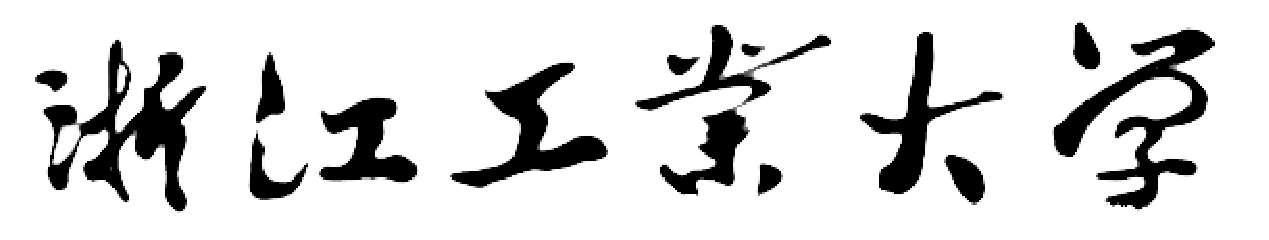
\includegraphics[width=9.84cm]{figures/zjut}
      \end{figure}
      \vspace*{9.66mm}
	  \song\yihao{本科毕业设计说明书(论文)}\\
	  \vspace*{10.0mm}
	  \song\xiaoer\bf{(2013届)}\\
      \vspace*{8.5mm}
      %校徽
      \begin{figure}[h]
        \centering
        
\includegraphics[width=2.73cm]{figures/zjutlogo}
      \end{figure}
      \vspace*{0.0mm}
      \renewcommand{\arraystretch}{1.0}
      \begin{tabular}{lc}
        \song\erhao{论文题目\quad} & \song\xiaoer{\@ctitle} \\ \cline{2-2}
      \end{tabular}\\
	  \vspace*{11.1mm}
      \setlength{\arrayrulewidth}{0.5pt}
      {\song\sihao
        \renewcommand{\arraystretch}{2.0}
        \begin{tabular}{lc}
          作者姓名\qquad &  \@cauthor \\ \cline{2-2}
          指导教师\qquad &  \@csupervisor \\ \cline{2-2}
          \\
          学科(专业)\qquad &  \@csubject \\ \cline{2-2}
          所在学院\qquad &  \@caffil \\ \cline{2-2}\cline{2-2}
          提交日期\qquad & \@cdate \\ \cline{2-2}
        \end{tabular}
	  }
    \end{center}
  \end{titlepage}

  %%%%%%%%%%%%%%%%%%% Abstract and Keywords  %%%%%%%%%%%%%%%%%%%%%%%
  \clearpage
  \markboth{摘~要}{摘~要}
  \addcontentsline{toc}{chapter}{摘~要}
  \setlength{\parskip}{24pt}
  \chapter*{\centering\hei\xiaoer{摘\qquad 要}}
  \setlength{\parskip}{18pt}
  \setcounter{page}{1}
  \song\defaultfont
  \setlength{\parskip}{0pt}
  \song\xiaosi{\@cabstract}
  \vspace{15pt}

  \hangafter=1\hangindent=52.3pt\noindent
  \hei\xiaosi\textbf{关键词:} \song\xiaosi{\@ckeywords}

  %%%%%%%%%%%%%%%%%%% English Abstract  %%%%%%%%%%%%%%%%%%%%%%%%%%%%%%
  \clearpage
  % \phantomsection
  \markboth{ABSTRACT}{ABSTRACT}
  \addcontentsline{toc}{chapter}{ABSTRACT}
  \setlength{\parskip}{24pt}
  \chapter*{\centering\tnroman\xiaoer\textbf{ABSTRACT}}
  \setlength{\parskip}{18pt}
  % \vspace{\baselineskip}
  \setlength{\parskip}{0pt}
  \@eabstract
  \vspace{15pt}

  \hangafter=1\hangindent=60pt\noindent
  \tnroman\xiaosi\textbf{Keywords:}  \tnroman\xiaosi{\@ekeywords}
}
\makeatother  % 格式设置
\graphicspath{{figures/}}  % 定义所有的eps文件在 figures 子目录下
% !Mode:: "TeX:UTF-8"
%%============================================================
%% 中文封面

\thispagestyle{empty}
\pdfbookmark[-1]{\zjuttitlec}{zjutthesiscover}
\phantomsection \label{zjutthesiscover}
\vspace*{4mm}
% 校名
\begin{center}
   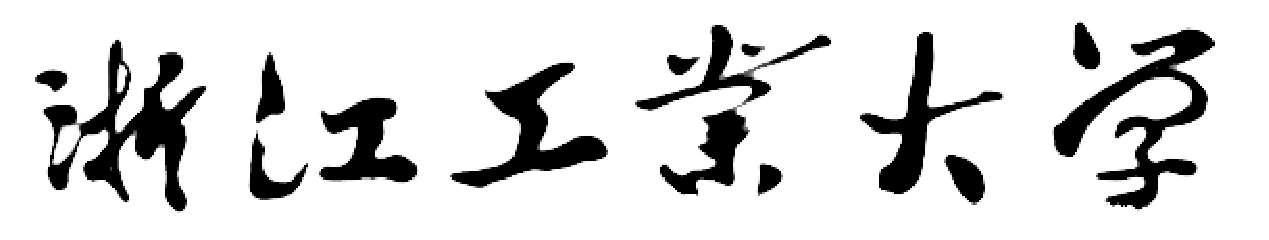
\includegraphics[width=98.40mm]{figures/zjut}
\end{center}
\vspace*{12mm}
\centerline{\songti\yihao{本科毕业设计说明书(论文)}}
\vspace*{8mm}
\centerline{\songti\xiaoer\textbf{(\zjutgrade\ 届)}}
\vspace*{7mm}
% 校徽
\begin{center}
  
\includegraphics[width=27.3mm]{figures/zjutlogo}
\end{center}

\vspace*{0.0mm}
\renewcommand{\arraystretch}{1.0}
\hspace*{12mm} 
{\songti\erhao{论文题目}}
\hspace{6mm} 
\begin{minipage}[t]{85mm} % 这里建议自行微调
    \linespread{1.1}{\songti\xiaoer\CJKunderline*{\zjuttitlec}}
\end{minipage}
\vspace*{1mm}
\begin{center}
    \setlength{\arrayrulewidth}{0.5pt}
    {\songti\sihao
        \renewcommand{\arraystretch}{1}
        \begin{tabular}{lc}
            作者姓名\qquad &  \zjutauthornamec \\ \cline{2-2}
            指导教师\qquad &  \zjutmentorc\\ \cline{2-2}
            \\
            学科(专业)\qquad &  \zjutmajor \\ \cline{2-2}
            所在学院\qquad &  \zjutcollegec \\ \cline{2-2}
            提交日期\qquad & \zjutsubmitteddatee \\ \cline{2-2}
        \end{tabular}
    }
\end{center}

  % 封面

\mainmatter\defaultfont\sloppy\raggedbottom

\begingroup % 在组内的chapter不换行
\let\clearpage\relax % chapter之后不换页
%%%%%%%%%% 摘要 %%%%%%%%%%
\titleformat{\chapter}{\centering\hei\sanhao\bfseries}{\chaptername}{1em}{} % 标题居中,黑体三号
%%%%% 标题 %%%%%
\chapter*{浙江工业大学本科生毕业设计开题报告模板}
\titleformat{\chapter}{\hei\sihao\bfseries}{\chaptername}{1em}{} % 恢复标题居左,黑体四号

%%%%%%%%%% 正文 %%%%%%%%%%
% !Mode:: "TeX:UTF-8"
\chapter{课题研究背景与意义}
掀起各国企业学习和运用的热潮。作为IE技术的基础运用,工作研究是最基本的技术,也是其他新兴IE技术运用的基础。企业在学习各种新的IE技术和\cite{2007}

\begin{equation}
\label{equaa5}
\iiint_1^1\frac{f(x)}{\sqrt{1-x^2}}dx = \frac{\pi}{n}\sum_{k=1}^nf(cos\frac{2k-4}{2n})+\frac{\pi}{2^{2n-1}(2n)!}f^{(2n)}(\theta)+max+\max
\end{equation}

张图片独自占一行的插入形式如\eqref{equaa5}~所示。

\chapter{课题研究的目标}
掀起各国企业学习和运用的热潮。作为IE技术的基础运用,工作研究是最基本的技术,也是其他新兴IE技术运用的基础。企业在学习各种新的IE技术和\cite{2007}

\begin{equation}
\label{equaa6}
\iiint_1^1\frac{f(x)}{\sqrt{1-x^2}}dx = \frac{\pi}{n}\sum_{k=1}^nf(cos\frac{2k-4}{2n})+\frac{\pi}{2^{2n-1}(2n)!}f^{(2n)}(\theta)+max+\max
\end{equation}

张图片独自占一行的插入形式如\eqref{equaa6}~所示。
% !Mode:: "TeX:UTF-8"

\chapter{研究开发的基本内容、目标,拟解决的主要问题或技术关键}
\section{研究目标}
在对比国内外教学质量工程申报评审系统的基本上,在研究国外内类似系统的设计实现上,提出自己的设计与实现。在当前教育优先发展的情况下,国家实施科教兴国战略,在这种情况下,教学质量当然也是非常重要的一个因素,关于如何提高教学质量,国家和学校都做了一些探索。特别在当信息技术如此普及的时代,借助信息技术来提高教学质量已是一种普遍的做法,国外已经在这方面走在了前头。本课题的研究目标定位于利用J2EE技术来实现教学质量工程申报评审系统的实现,特别是应用J2EE中的一些关键技术和框架,如Hibernate、Spring、Spring MVC。

\section{研究的基本内容}
由于整个系统的结构庞大,开发工作量大,所以本研究的基本内容并不定位于整个系统的设计与实现上。相反,本研究的基本内容是教学质量工程申报评审系统中的申报子系统功能模块上。
申报子系统的主要功能是根据教育厅发布的项目申报指南和限额,项目申报单位(学校)组织本校教师集中进行项目的申报及对项目的初审。
本研究的具体容包括:

(1)	信息发布\par
信息发布的主要功能是申报通知、申报指南等信息发布,主要是文字内容和相关文档附件。发布信息只能由教育厅主管部门人员进行。对于撰写完毕的信息,可以存入草稿箱中,等待用户修改后发布。对信息提供添加、删除、修改功能。

(2)	项目申报\par
项目申报的主要功能是项目申报人根据学校分发的项目申报密钥进行项目申报书的填写。申报项目的类型和项目的名称已由学校事先录入,申报人不得更改。申报人需要填写在线项目申报简表,上传项目申报书(PDF格式)。填写中可对内容保存、提供修改功能。最后,把申报简表和申报书一起提交到学校。

项目的申报是项目申报子系统中的一个重要的功能,也是该子系统的核心功能。主要包括两大模块填写申报书和提交申报书。

申报人必须按规定在线填写申报简表,按申报书要求离线填写项目申报书,然后把申报简表和项目申报书提交学校。项目的名称和类别已经由学校指定,申报人不得修改;如需修改,必须由学校进行修改。
项目申报信息的填写可以中途保存或填写完毕后提交。提交的申报项目将不能修改。在项目申报的有效时间段内,用户都可以凭密钥登陆系统。项目申报书提交后就不能修改,但可查阅。系统不设置自动提交项目申报材料功能,提交工作由申报人手工操作,并进行确认。

申报简表和申报书核对无误后,申报人把申报简表和项目申报书提交到学校。项目申报书提交后就不能修改,若要修改,需要由学校先进行退回操作。

(3)	学校申报管理\par
各申报单位(学校)负责管理本单位的项目申报工作,并对项目进行初审。学校根据教育厅下达的种类项目的申报限额和申报截止时间,建立本校的具体申报项目和相应的用户密钥,完成本校申报项目的初审并报送教育厅。若申报时间逾期,学校将不能向教育厅提交项目申报,除非教育厅给予再次授权开通。学校在向教育厅正式提交项目申报前,可对申报人所提交的申报材料进行查阅、审核,可以把申报材料退回申报人进行修改,但当正式提交教育厅后,就不能再对申报材料进行修改操作。

在申报系统中,每个学校只能查看本校申报的项目。

新建申报项目。学校在教育厅所授权指定的项目类型中进行项目申报的新建。新建的申报项目数量不得超过教育厅设定的本校申报限额。新建申报项目需要指定项目的名称、项目所属的学科门类(便于项目分组和专家匹配)和指定申报用户密钥。对新建项目申报以列表形式显示,并标示为待填报状态。列表显示新建申报项目的公共属性(如项目类型、项目所属学科门类、项目申报人、用户名)。教师申报用户凭学校分发的密钥进行项目申报书的填写。申报系统对列表中的新建申报项目,提供查看、修改、删除操作。

待初审项目。在申报用户提交后,项目即转入等初审状态。学校对申报项目进行初审,对需要修改的申报项目,可以退回申报人进行修改。

初审通过项目。对初审通过的项目,标示状态为初审通过。对初审通过的项目,提供同类别申报项目的整批提交操作。系统不提供逐个项目单独提交的功能。系统提供对初审项目的优先排序等特殊标记功能。
已提交项目。向教育厅提交的本校申报项目。对已经提交的项目标示已提交教育厅的状态。对项目的提交,只允许提交一次,且前提条件为提交项目的总数不得超过限额,对于小于限额数量的提交操作,给出提醒信息。若一次提交了部分项目,之后又要再提交一些项目,则需要管理员将已经提交的项目退回,申报单位一次性提交全部项目。

(4)	申报设定\par
申报设定的主要功能是对项目申报类别和每个类别各学校相应申报数量的管理。只有启用的申报类别,在学校申报管理中出现。同时可以启用多个申报类别。设定每个申报类别的申报评审时间限制。

\section{需要解决的技术难点}
Spring MVC,Hibernate,Spring框架的整合使用。\par
Ajax技术的使用。\par
密钥的生成与管理。\par

% !Mode:: "TeX:UTF-8"

\chapter{研究开发的方法、技术路线和步骤}
(1)	系统平台:Microsoft Windows XP

(2)	系统构架:B/S构架\par
B/S(Browser/Server)结构即浏览器和服务器结构。它是随着Internet技术的兴起,对C/S结构的一种变化或者改进的结构。在这种结构下,用户工作界面是通过WWW浏览器来实现,极少部分事务逻辑在前端(Browser)实现,但是主要事务逻辑在服务器端(Server)实现,形成所谓三层3-tier结构。这样就大大简化了客户端电脑载荷,减轻了系统维护与升级的成本和工作量,降低了用户的总体成本(TCO)。以目前的技术看,局域网建立B/S结构的网络应用,并通过Internet/Intranet模式下数据库应用,相对易于把握、成本也是较低的。它是一次性到位的开发,能实现不同的人员,从不同的地点,以不同的接入方式(比如LAN, WAN, Internet/Intranet等)访问和操作共同的数据库;它能有效地保护数据平台和管理访问权限,服务器数据库也很安全。用户在局域网各工作站通过WWW浏览器就能实现工作业务。特别是在JAVA这样的跨平台语言出现之后,B/S架构管理软件更是方便、快捷、高效。

(3)	编程语言:JAVA\par
JAVA语言是SUN公司于1995年推出的一种面向对象的新一代程序。到现在JAVA已经成为主流的开发语言之一,其应用领域带在继续扩大。特点:

{\kai 第一、面向对象,他是更加彻底的面向对象,面向对象的特点使设计集中于对象及其对象之间的联系。JAVA中提供了简单的类机制和动态接口模型,使对复杂系统的设计更加简单、清晰。

第二、平台无关性,用JAVA写的应用程序不用修改就可在不同的软硬件平台上运行。

第三、可靠性和安全性,由于JAVA主要用于网络应用程序开发,因此对安全性有较高的要求。如果没有安全保证,用户从网络下载程序执行就非常危险。JAVA通过自己的安全机制防止了病毒程序的产生和下载程序对本地系统的威胁破坏。当JAVA字节码进入解释器时,首先必须经过字节码校验器的检查,然后JAVA解释器将决定程序中类的内存布局,随后,类装载器负责把来自网络的类装载到单独的内存区域,避免应用程序之间相互干扰破坏。最后,客户端用户还可以限制从网络装载的类只能访问某些文件系统。上述几种机制结合起来,使得JAVA成为安全的编程语言。

第四、	JAVA还有分布性、多线程、高效性和动态性等优点。}

(4)	所用架构:Spring MVC+Hibernate+Spring\par
Spring MVC是一个基于MVC模式的Web应用程序的框架。现已逐渐成为开发Web应用程序的主流框架。在继承 MVC模式的各种特征的基础上,根据J2EE的特征进行了相应的变化和扩展。

业务层通过Hibernate进行数据库操作。Hibernate通过读取配置文件(hibernate.cfg.xml)和类的映射文件(xmlMapping)中的内容, 生成SessionFactory实例的工厂,由它的openSession()方法负责每次所需的Session对象的创建,在Session对象的方法中借助持久化对象(persistent object)来完成对数据库的操作,而不须使用JDBC和SQL进行数据的操作。

系统应用Spring框架来简化系统的配置,管理系统中的bean和简化Hibernate的连接过程。

(5)	服务器软件:JBOSS\par
JBoss是全世界开发者共同努力的成果,一个基于J2EE的开放源代码的应用服务器。因为JBoss代码遵循LGPL许可,你可以在任何商业应用中免费使用它,而不用支付费用。Jboss支持EJB 1.1和EJB 2.0的规范,它是一个为管理EJB的容器和服务器。类似于Sun's J2SDK Enterprise Edition(J2EE),Jboss的目标是一个源代码开放的J2EE环境。但是Jboss核心服务仅是提供EJB服务器。JBOSS不包括serverlers/JSP page 的WEB容器,当然可以和Tomcat或Jetty绑定使用。

(6)	系统开发工具:MyEclipse\par
MyEclipse是一个优秀的开发环境,它提供的核心框架和可延伸的外挂程式机制给广大的程序设计师提供了无限的想象和创造空间。目前网上流传相当丰富且全面的开发工具方面的外挂程式,但是MyEclipse已经超越了开发环境的概念,可以想象MyEclipse将成为未来的整合的桌面环境。目前的MyEclipse本身就具有资源管理和外部程式的功能,加上无所不能的外挂程式,将构成一个丰富多彩的工作环境而不仅仅是一个IDE。

(7)	数据库软件: Oracle 11g\par
Oracle 11g是Oracle公司推出的一款功能强大的数据库管理系统,方便用户的数据库操作。

% !Mode:: "TeX:UTF-8"

\chapter{研究工作总体安排与时间进度}
\begin{table}[!h]
\vspace{0.5em}\centering\xiaosi
\begin{tabular}{|c|c|c|}
\toprule[1.5pt]
任务序号 & 起止时间 & 阶段任务要点 \\
\midrule[1pt]
1 & 2010.11.30-2011.1.20 & \tabincell{c}{了解课题相关内容,查找中、\\英文资料} \\\hline
2 & 2011.1.21-2011.3.11 & \tabincell{c}{查阅文献资料,完成文献综述、\\开题报告和外文翻译} \\\hline
3 & 2011.3.12-2011.3.20 & \tabincell{c}{学习Spring、Hibernate、Ajax\\等开发相关技术} \\\hline
4 & 2011.3.21-2011.3.31 & 分析需求,确定开发工具 \\\hline
5 & 2011.4.1-2011.4.5 & 进行系统的概要设计 \\\hline
6 & 2011.4.6-2011.4.15 & 进行系统的详细设计 \\\hline
7 & 2011.4.16-2011.4.20 & 系统框架及开发环境搭建 \\\hline
8 & 2011.4.21-2011.5.21 & 进行项目的开发 \\\hline
9 & 2011.5.22-2011.5.25 & 完成系统测试 \\\hline
10 & 2011.5.26-2011.6.5 & 整理资料、完成毕业论文 \\\hline
11 & 2011.6.5-2009.6.10 & 上交毕业论文、准备毕业答辩 \\
\bottomrule[1.5pt]
\end{tabular}
\end{table}


\endgroup % 组结束
%%%%%%%%%% 参考文献 %%%%%%%%%%
\clearpage % 显式换页,使书签定位准确
\defaultfont
\bibliographystyle{GBT7714-2005NLang-ZJUT}
\phantomsection
\markboth{参考文献}{参考文献}
\addcontentsline{toc}{chapter}{参考文献}       % 参考文献加入到中文目录
\nocite{*}                                     % 若将此命令屏蔽掉,则未引用的文献不会出现在文后的参考文献中。
\bibliography{references/reference}

\end{document}
